\documentclass[b5paper,10pt]{article}
\usepackage[colorlinks]{hyperref}
\usepackage{graphicx}
\usepackage{tikz-cd}
\usepackage{notestemplate}
\title{Motivic Homotopy Theory}
\author{Chow.}
\begin{document}
\maketitle
\tableofcontents
	\section{Construction of Unstable Homotopy Category}
	In order to refine the triangulated category of Voevodsky's motives and apply more tools from algebraic topology, we need well-behaved homotopy theory for schemes. Homotopy theory for schemes also allow us to construct motivic cohomology and algebraic K-theory which are looked as generalized cohomology theory defined with Brown representativity theorem.
	\subsection{Simplicial Sheaves and Hypercovers}
	Let us firstly recall some simplicial homotopy theory.
	$\Delta$ is category consists of objects such as
	\[
	[n]={0 \to 1 \to 2 \to \cdots \to n}
	\]
	for all non-negative integer $n$. And morphisms are functions of sets preserving the order of arrows.
	The category of \emph{simplicial sets} means the category of presheaves on $\Delta$ with values over $\mathbf{Sets}$. It is denoted by $\mathbf{sSets}$.
	
	In category of simplicial sets, we have following canonical objects
	\[
	\Delta[n] := \Delta(-,[n])
	\]
	They are call \emph{standard simplicial sets}.
	\begin{secprop}
		$\Delta([m],[n])$ is generated by following morphisms
		\[
		\begin{aligned}
			d^i \colon [k] &\to [k+1]\\
			d^i(0 \to 1 \to 2 \to \cdots \to k)&=\begin{cases}
			1\to 2 \to \cdots \to k+1& \text{if } i =0\\
			0 \to 1 \to \cdots \to i-1 \to i+1 \to \cdots \to k+1& \text{if } 1\leq i \leq k\\
			0 \to 1 \to \cdots \to k& \text{if } i =k+1\\
			\end{cases}
		\end{aligned} 
		\]
		and
		\[
		\begin{aligned}
		s^i \colon [k] &\to [k-1]\\
		s^i(0 \to 1 \to 2 \to \cdots \to k)&=\begin{cases}
		0\to 0 \to 1 \to \cdots \to k-1& \text{if } i =0\\
		0 \to \cdots \to i \to i  \to \cdots \to k-1& \text{if } 1\leq i \leq k-1\\
		\end{cases}
		\end{aligned} 
		\]
		where $d^i$ is called co-face map and $s^i$ is called co-degeneracy map.
	\end{secprop}
$\Delta$ is small category. As diagram, $\Delta$ looks like
\[
\begin{tikzcd} 
 {[0]} \arrow[r, shift left,"d^0"] \arrow[r, shift right,"d^1"'] & {[1]} \arrow[r,"d^0" description] \arrow[r, shift left=4,"d^1"] \arrow[r, shift right=4,"d^2"'] & \cdots 
\end{tikzcd}
\]
\[
\begin{tikzcd} 
{[0]} \arrow[r,"s^0",leftarrow] & {[1]} \arrow[r,shift left,"s^0",leftarrow] \arrow[r, shift right,"s^1"',leftarrow]  & \cdots 
\end{tikzcd}
\]
By Yoneda lemma, for simplicial set $X \in \mathbf{sSets}$, we have 
\[
X([n])\simeq \mathbf{sSets}(\Delta[n], X)
\]
For convenience, we always denote $X([n])$ by $X_n$ for simplicial set $X$, $d_i = X(d^i)$ and $s_i= X(s^i$). 
\begin{figure}[h]
	\caption{Idea of simplicial sets (from ncatlab)}
\centering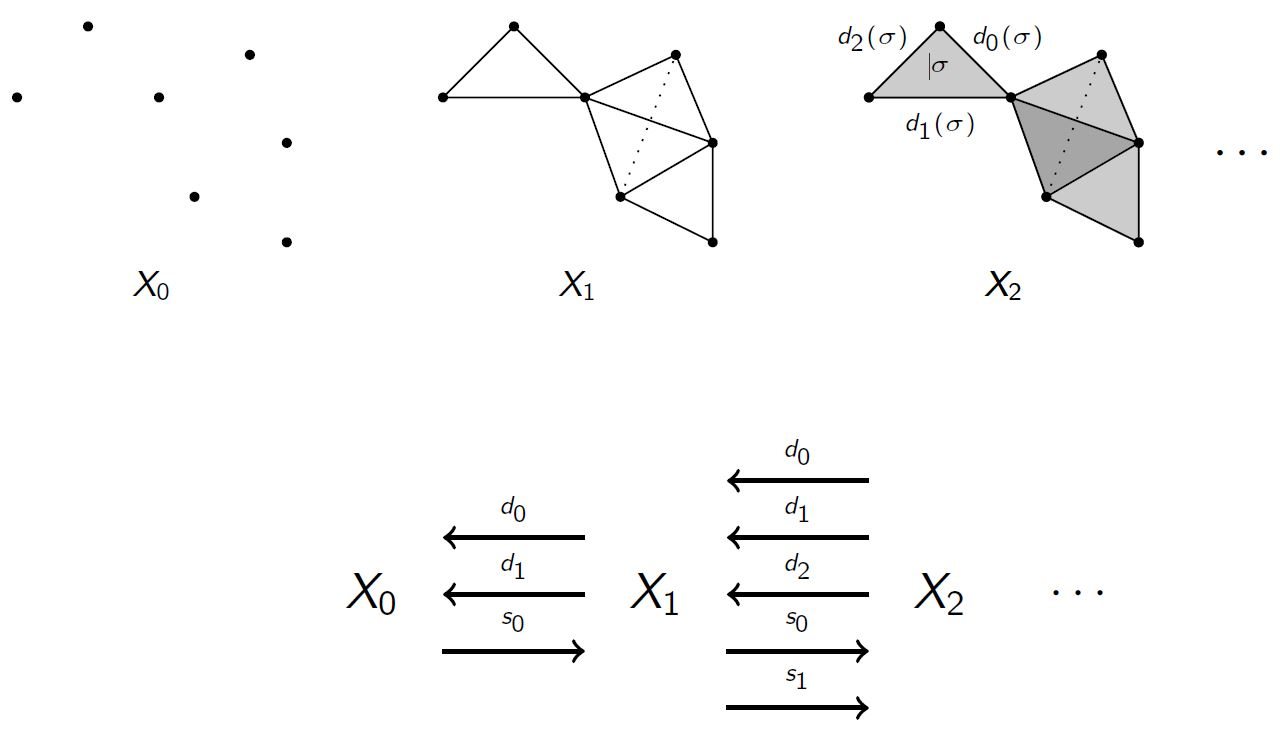
\includegraphics[scale=0.5]{PIC/SimplicialSetsIdea.jpg}
\end{figure}

Let $\Delta^n$ be standard simplex in topological space category. Then we can defined topological space respect to given simplicial set $X$ as follows
\[
|X| := \colim_{(\Delta_n \to X) \in \mathbf{sSets}/X} \Delta^n
\]
Furthermore, $|-|$ is covariant functorial in $\mathbf{sSets}$ since co-representable $\mathbf{sSets}(\Delta_n,-)$ and colimit are functorial. $|-|$ is called \emph{geometric realization functor}.

In classical simplicial homotopy theory, we can endow $\mathbf{sSets}$ with model structure where fibrations are Kan fibrations and weak equivalence are morphisms which induce isomorphisms between fibrant objects on homotopy groups (can be defined as homotopy groups of corresponding geometric realizations).
\subsubsection{Simplicial Objects}
Let $\mathcal{C}$ be arbitrary category. We say $X_*$ is a \emph{simplicial object} on $\mathcal{C}$ if $X_*$ is a presheaf $X_* \colon \Delta^{op} \to \mathcal{C}$ and $\mathbf{s}\mathcal{C}$ denotes the category of simplicial objects on $\mathcal{C}$. Hence simplicial sets are simplicial objects on $\mathbf{Sets}$. 

If $\mathcal{A}$ is  an Abelian category, then we have following correspondence
\begin{secprop}[Dold-Kan Correspondence]
\[
N \colon s\mathcal{A} \to \mathbf{Ch}_{\geq 0} (\mathcal{A})
\]
is Quillen equivalence (i.e.\ category equivalence which is also Quillen functor) respect to canonical model structure on $s\mathcal{A}$ and projective model on $\mathbf{Ch}_{\geq 0 } (\mathcal{A})$. $N$ is functor of normalized complex and $\mathbf{Ch}_{\geq 0}(\mathcal{A})$ is category of non-negative chain complexes. This equivalence is called \emph{Dold-Kan correspondence}.
\end{secprop}
This proposition means that homological algebra over Abelian category in low bounded case is equivalent to homotopy theory for its simplicial objects. It is convenient to study homotopy theory for simplicial objects because we have geometric realization functor to make constructions more natural. So we can transplant properties from classical homotopy theory into homological algebra.
\subsubsection{Simplicial Homotopy Theory for Presheaves and Sheafification}
Suppose $\mathbf{PSh}(\mathcal{C})$ be the category of presheaves on $\mathcal{C}$.

\end{document}